\documentclass[10pt]{article}
\usepackage[utf8]{inputenc}
%\usepackage[T1]{fontenc}
\usepackage{tgbonum}
\usepackage[english]{babel}
\usepackage{graphicx}
\usepackage{amsmath}
\usepackage{amssymb}
\usepackage{hyperref}
\usepackage{epsf}
\usepackage{float}
\usepackage{mathpazo}
\usepackage{pifont}
\usepackage
[
a4paper,% other options: a3paper, a5paper, etc
left=2.2cm,
right=2.2cm,
top=3cm,
bottom=3cm,
]{geometry}
%\geometry{hmargin=3.5cm, vmargin=2.5cm}
\usepackage{fancyhdr}
\pagestyle{fancy}
\fancyhf{}
\rfoot{\thepage}
\renewcommand{\headrulewidth}{0pt}
\usepackage{color}
\graphicspath{{DWGs/}}
\usepackage{graphicx}
\usepackage{wrapfig}
\usepackage{graphicx}
\usepackage{multicol}
\usepackage{enumitem}
\usepackage{xcolor}
\usepackage{framed}
\definecolor{shadecolor}{RGB}{139, 231, 3}
\usepackage{epigraph}
\usepackage{bm}
\usepackage{tcolorbox}
\definecolor{mycolor}{rgb}{0.122, 0.435, 0.698}

\newtcbox{\mb}{nobeforeafter,colframe=mycolor,colback=mycolor!10!white,boxrule=0.5pt,arc=4pt,
  boxsep=0pt,left=6pt,right=6pt,top=3pt,bottom=3pt,tcbox raise base}

\usepackage{eso-pic}
\newcommand\BackgroundPic{%
\put(-50,-0){%
\parbox[b][\paperheight]{\paperwidth}{%
\vfill
\centering

\includegraphics[height=\paperheight,%
keepaspectratio]{DWGs/cover.png}%
\vfill
}}}

\usepackage{emerald}
\usepackage[T1]{fontenc}

\usepackage{anyfontsize}
\usepackage{t1enc}
\newcommand{\heart}{\ensuremath\varheartsuit}
\usepackage{tikz}
\usetikzlibrary{positioning}

\usepackage{xcolor}

\newcommand{\highlight}[1]{%
  \colorbox{blue!50}{$\displaystyle#1$}}

\begin{document}

\begin{titlepage}
    \begin{center}

		\vspace*{7cm}    

        \Huge
        \textbf{Flow types}
        
        
        \vspace*{0.5cm}
        
        \Large


		\Large

        \vspace{2cm}
        
        \LARGE

        K. Zdybal

        \vspace{10.5cm}
        
		\Large

 		August, 2018
	\end{center}
\end{titlepage}

% EX LIBRIS PAGE ================================================

\thispagestyle{empty}
\begin{center}
\vspace*{4cm}
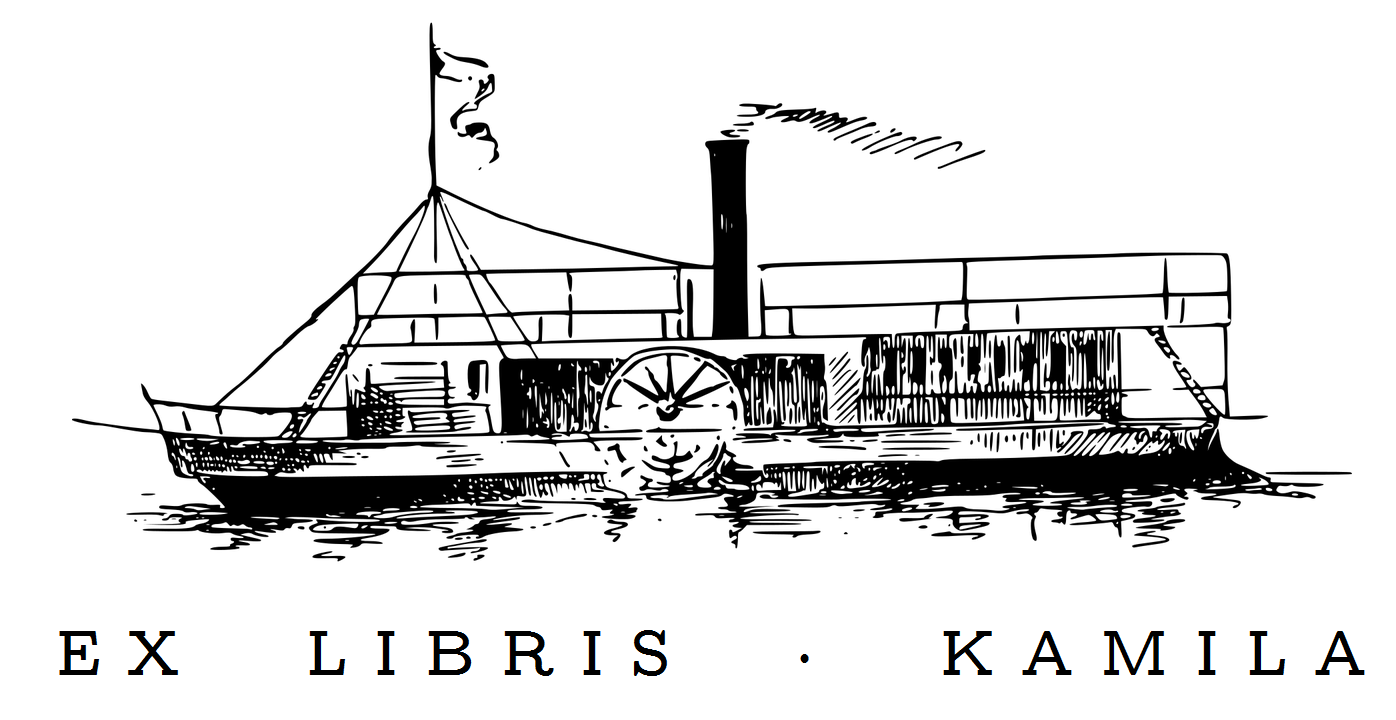
\includegraphics[width = 80mm]{ex_libris.png}

\vspace*{2cm}

Copyright \textcopyright \, K. Zdybał, 2018

For more projects similar to this one

visit me on GitHub: \verb|@camillejr|

\verb|camillejr.github.io/science-docs/|

To contact me personally drop me a line at:

\verb|kamilazdybal@gmail.com|

\vspace*{2cm}

\verb|Flow types|

\verb|version 1.0|

Typeset with \ding{170} for \LaTeX

\vspace*{1.8cm}

\noindent This work is licensed under the Creative Commons

Attribution-NonCommercial-ShareAlike 4.0 International 

(CC BY-NC-SA
4.0) license.
\end{center}

\setlength{\parindent}{0cm}
\clearpage

\tableofcontents

\setlength{\parskip}{1em}
\renewcommand{\baselinestretch}{1.0}

\section{Introduction}\label{chap:motivation}



\section{Poiseuille flow with constant pressure gradient}

\subsection{Derivation}

Let us consider an infinitesimal fluid element.

\subsubsection{Assumptions}

The following assumptions are made in the derivation:

\begin{enumerate}
\item Fluid is Newtonian, hence obeys the law:
\begin{equation}
\tau_{yx} = -\mu \frac{du}{dy}
\end{equation}
\item Pressure gradient is constant:
\begin{equation}
\frac{dp}{dx} = \text{const}
\end{equation}
\item Only one velocity component $u$ is non-zero and hence the motion only happens in the $x$-direction.
\end{enumerate}




\subsubsection{Sign convention}

The sign of the shear stress $\tau_{yx}$ is positive when it is the shear exerted by the fluid element with a smaller $y$-coordinate on a fluid element with a larger $y$-coordinate.

The sign of the pressure $p_x$ is positive when it is the pressure exerted by the fluid element with a smaller $x$-coordinate on a fluid element with a larger  $x$-coordinate.




\subsection{A note for the curious minds}

It is interesting to pause for a moment and ponder about the nature of the differential world. Notice that the sole thing we did to get us to arrive at the final formula for the velocity distribution was to consider an infinitesimal element from the "inside" of the channel. We picked a place that is "nothing special", through which we mean that it is the most generic possible fluid element and not, for instance, a fluid element at the very boundary. Writing the momentum balance for that infinitesimal fluid element and integrating to generalize for every fluid element and then applying the boundary conditions, we obtain a solution that holds for \textbf{any} fluid element in the cross-section! It must be one of the amazing results of differential calculus: starting from an element that is so small it's hard to even believe in their efficacy, we obtain a result that might be used for channels that are tens of centimeters in diameter.

There is one more interesting thing that I would like to point out. Notice that all "types" of fluid elements that can happen throughout the channel cross-section are taken into account in the final result for velocity distribution. And in the Poiseuille flow presented above there really are only three types! There is the most generic type from the inside of the channel for which we wrote the momentum balance - this is a fluid element which is surrounded from all sides by more fluid. There is the second type of fluid element which is bounded from below and in order to include it in the final solution we incorporated the boundary condition for the bottom wall. And there is the third type which is bounded from above for which we also wrote one more boundary condition applicable at the top wall. That is all the information we needed to cover all possible fluid elements in the whole depth of the channel.



\section{Uniform flow}




\section{Couette flow}



\section{Gravity-driven flow}


\begin{thebibliography}{3}

\item 

\end{thebibliography}

\end{document}
